\section{Examples}
\subsection{Code-Example}
To demonstrate a race condition, snippet \ref{list:simple_race_condition} shows a program, which increments a global (reachable anywhere in the program) variable 1 million times (high number here to greater-display disparity), but also concurrently decrements the same counter 1 million times. After this the program outputs the final value of \texttt{counter}.

\begin{lstlisting}[language=C++, caption={Program displaying race condition, modifying a global counter.}, label=list:simple_race_condition]
#include <iostream> //printing to stdout
#include <thread> //setting up threads

int counter = 0; //global var.

void increment() { //function to increment the global counter 1m. times; 1m. here to further demonstrate greater disparity from race condition inherently present here
    for (int i = 0; i < 1000000; i++) { //1m. loop
        counter++; //increment counter
    }
}

void decrement() { //same as increment but will decrement the counter 1m. times
    for (int i = 0; i < 1000000; i++) {
        counter--;
    }
}

int main() { //driver code to call each increment, decrement function on separate threads
    std::thread thread1(increment);
    std::thread thread2(decrement);
    thread1.join(); //'join' forces whichever thread finished first to wait on the other
    thread2.join();
    std::cout << "Counter: " << counter << std::endl; //print the final val. of counter
    return 0;
}
\end{lstlisting}
The output from the program shown in snippet \ref{list:simple_race_condition} (run 5 times) is observable in figure \ref{fig:race_condition_output}, showing the wildly differing values of counter per-time the program is run.
\begin{figure}[!htbp]
    \centering
    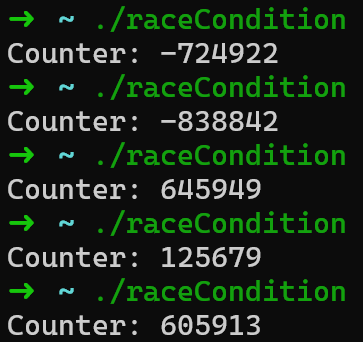
\includegraphics[scale=.5]{figures/simple_race_condition_program_output.png}
    \caption{Output of program from snippet \ref{list:simple_race_condition} run 5 times}
    \label{fig:race_condition_output}
\end{figure}

\subsection{Producer-Consumer Problem}
\label{producer_consumer}
In this problem, there are two processes, producer and the consumer.\\
The producer's role is to fill a shared resource: a fixed-size buffer.\\
The consumer's role is to transfer data from the shared buffer elsewhere (perhaps elsewhere in the consumer's memory region).\\
Since the buffer is fixed-size (cannot grow/shrink), more data than can 'fit' in the buffer cannot be allowed (from the producer) (buffer overflow; undefined behaviour), further, more data than is in the buffer cannot be transferred from the buffer (by the consumer) (buffer underflow; undefined behaviour).\\
Henceforth, the solution must involve some synchronisation primitive to the buffer.\\
This problem is present due to the nature of concurrency, since if the producer is running on a different thread to the consumer, the two threads are likely not operating at identical clock-speeds (assuming threads running on different cores (CPUs)\footnote{However, even running on a machine with one-core, two-threads, race-conditions can still be present due to half a transaction occurring on \texttt{T1} then switching to \texttt{T2}, which are both modifying same data; not true concurrency, however atomicity is \textbf{not} guaranteed as a result of this.}), and even so, the load on each is likely to be different on an ordinary consumer-system\footnote{As opposed to a specialised-OS, wherein one process might be exclusively-allocated an entire core (CPU).}.\\
Furthermore, if each producer and consumer can access the buffer concurrently, the consumer may begin transferring data from the shared buffer before the producer has finished emplacing the data in the buffer; if this happens some (say half) of the data in the buffer have been 'consumed' by the consumer, but the remaining data may not, and this region may be marked as 'complete', or similar, as such there is some corruption of data shared between the two processes in this way. One solution to this, however, more solutions will be covered in Section \ref{solutions}, is for each the producer and consumer to 'signal' the other upon performing their respective operation, e.g. producer emplacing some data.